\chapter{Gradients of all architectures - original setting (non-shifted)}\label{appendixA}


\section*{Velocity}\label{sec:velocity-appendixA}

\subsection*{Full dataset}\label{subsec:vel-full-dataset-appendixA}
\begin{figure}[!htb]
\centering
\begin{subfigure}[a]{\textwidth}
   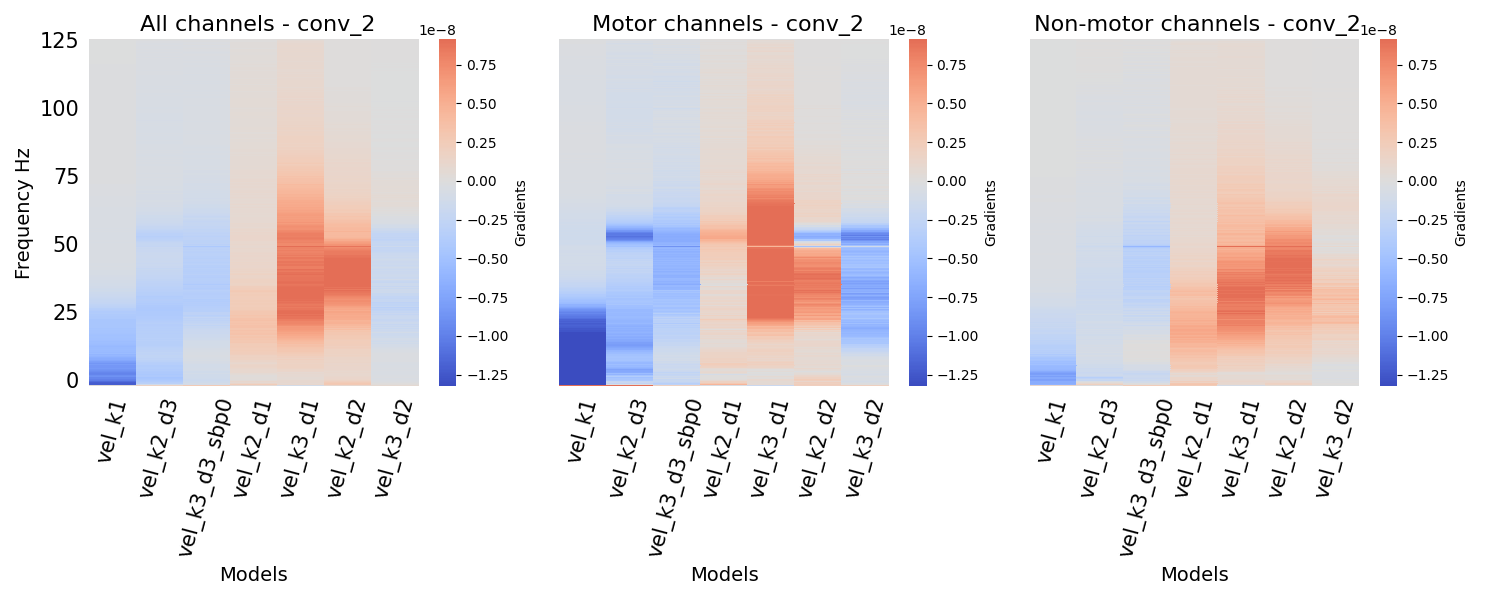
\includegraphics[width=0.85\linewidth]{img/appendix/A/conv-2/m/vel-model-gradients-all_kinds}
   \caption{}
   \label{fig:vel-full-grads-conv2}
\end{subfigure}

\begin{subfigure}[b]{\textwidth}
   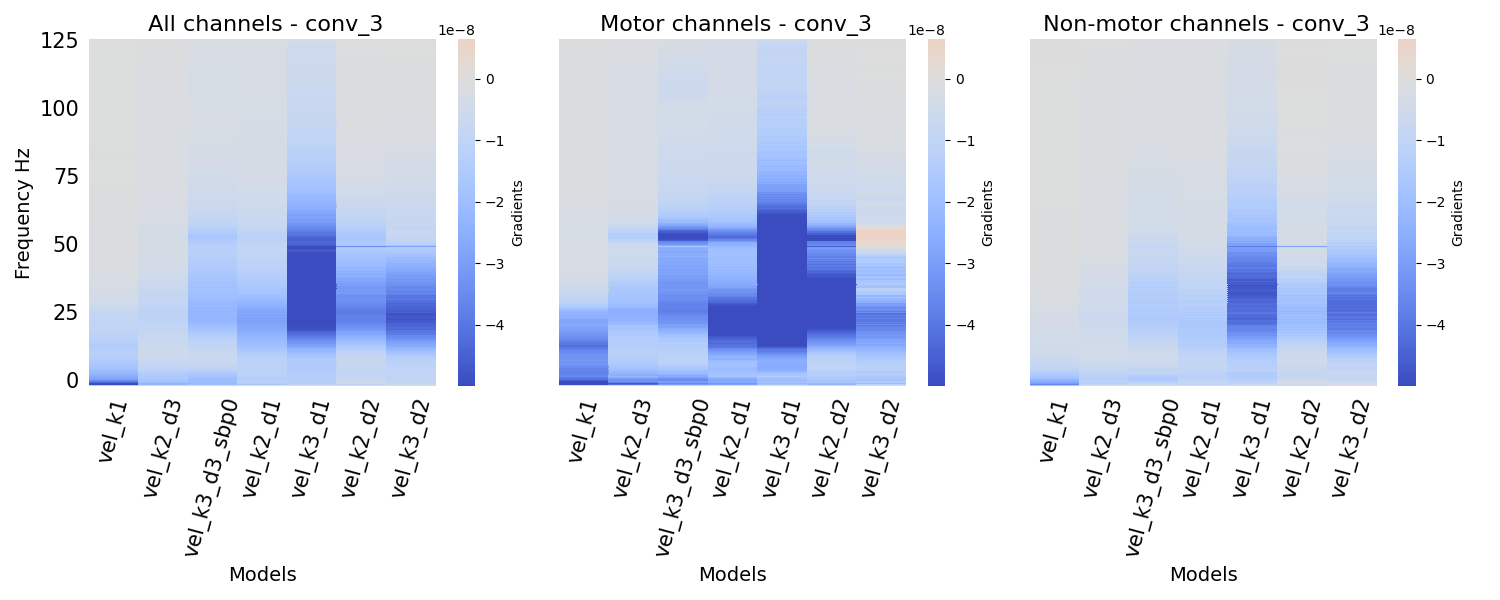
\includegraphics[width=0.85\linewidth]{img/appendix/A/conv-3/m/vel-model-gradients-all_kinds}
   \caption{}
   \label{fig:vel-full-grads-conv3}
\end{subfigure}
\end{figure}
\clearpage   

\begin{figure}[!htbp]\ContinuedFloat
\begin{subfigure}[c]{\textwidth}
   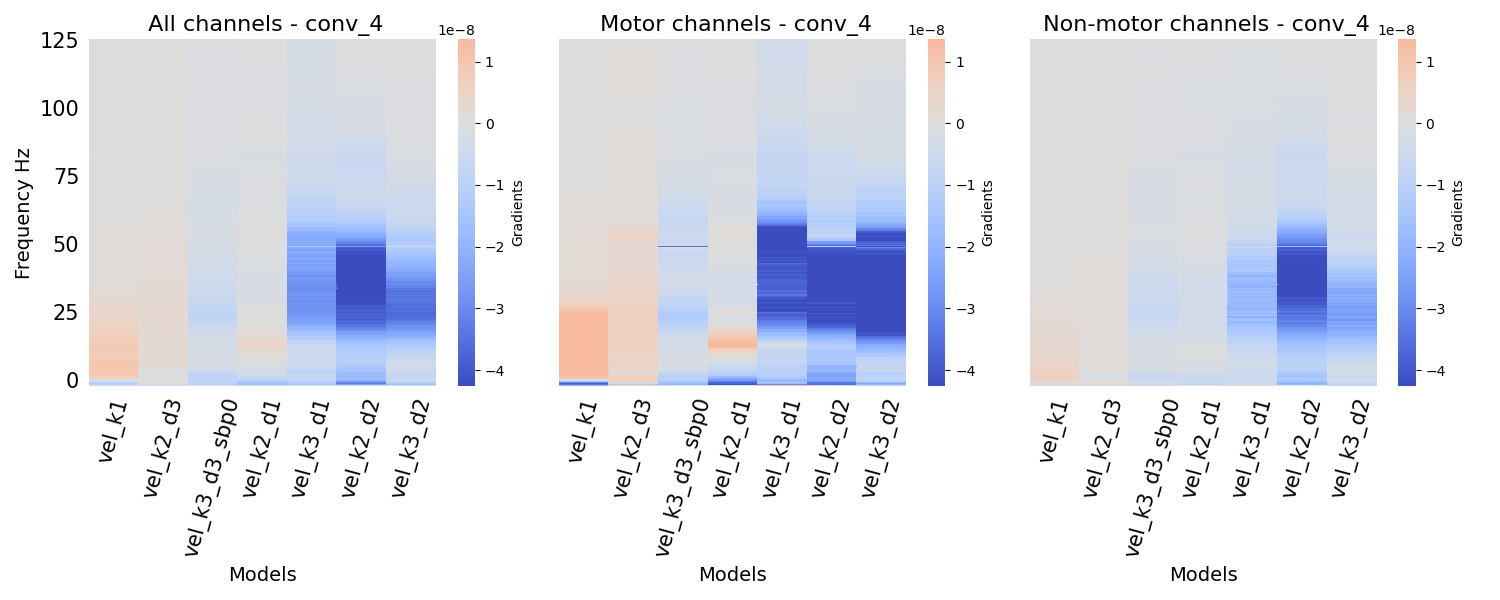
\includegraphics[width=0.9\linewidth]{img/appendix/A/conv-4/m/vel-model-gradients_all_kinds}
   \caption{}
   \label{fig:vel-full-grad-covn4}
\end{subfigure}

\begin{subfigure}[d]{\textwidth}
   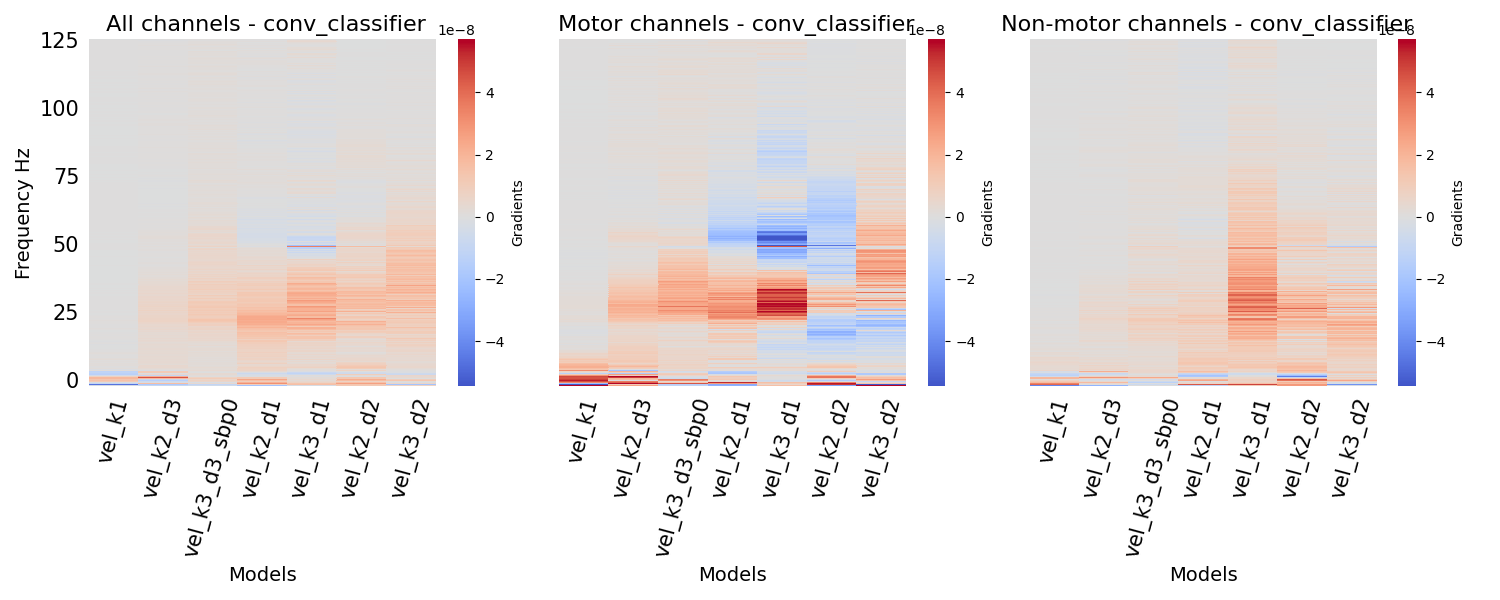
\includegraphics[width=0.9\linewidth]{img/appendix/A/conv-classifier/m/vel-model-gradients_all_kinds}
   \caption{}
   \label{fig:vel-full-grads-conv-classifier}
\end{subfigure}

\caption[]{Gradients of the different CNN architectures decoding velocity from the full dataset in the original non-shifted setting (causal prediction). \textbf{(a)} shows gradients of the convolutional layer in the second block; \textbf{(b)} shows gradients of the convolutional layer in the third block; \textbf{(c)} shows gradients of the fourth convolutional block; \textbf{(d)} shows gradients of the last convolutional layer - the output layer. All channels include channels that do not belong to motor neither non-motor channel sets. See Section \ref{subsec:ieeg-data-preprocessing}}
\label{fig:vel-full-grads}
\end{figure}
\clearpage
\subsection*{High-passed dataset}\label{subsec:vel-high-passed-dataset-appendixA}
\begin{figure}[!htb]
\centering
\begin{subfigure}[a]{\textwidth}
   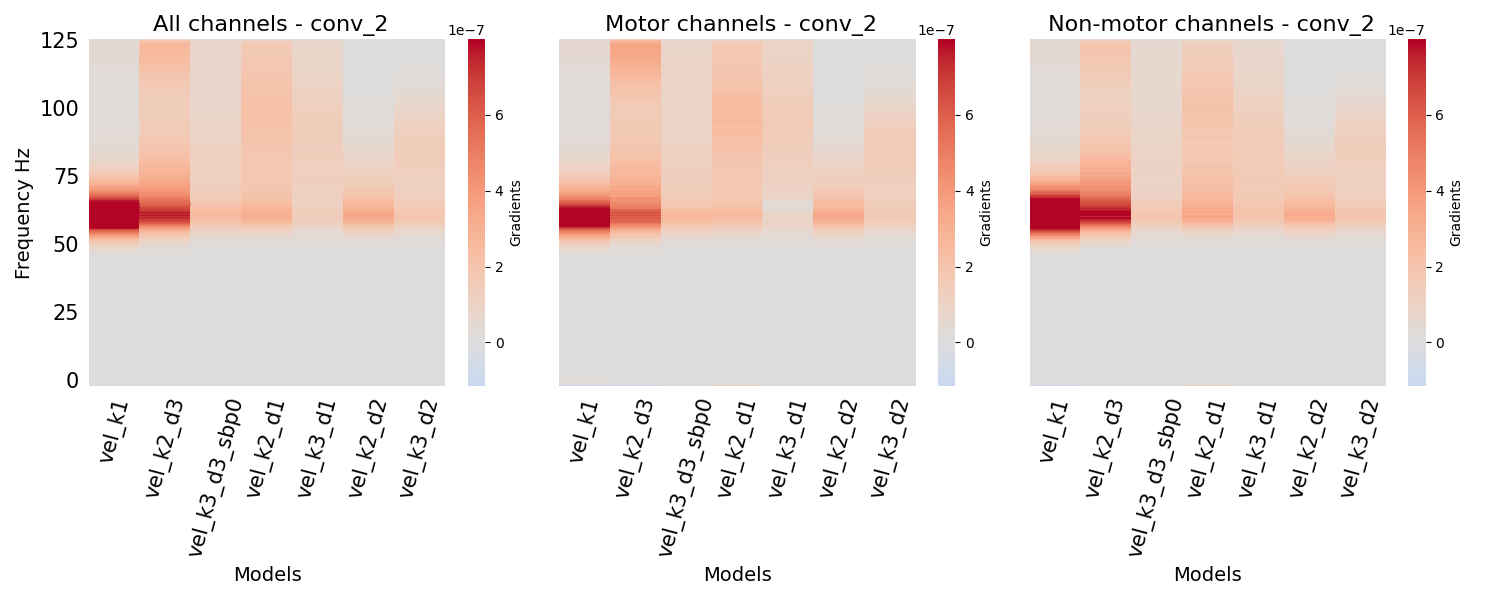
\includegraphics[width=0.9\linewidth]{img/appendix/A/conv-2/hp-m/vel-model-gradients_all_kinds}
   \caption{}
   \label{fig:vel-hp-grads-conv-2}
\end{subfigure}

\begin{subfigure}[b]{\textwidth}
   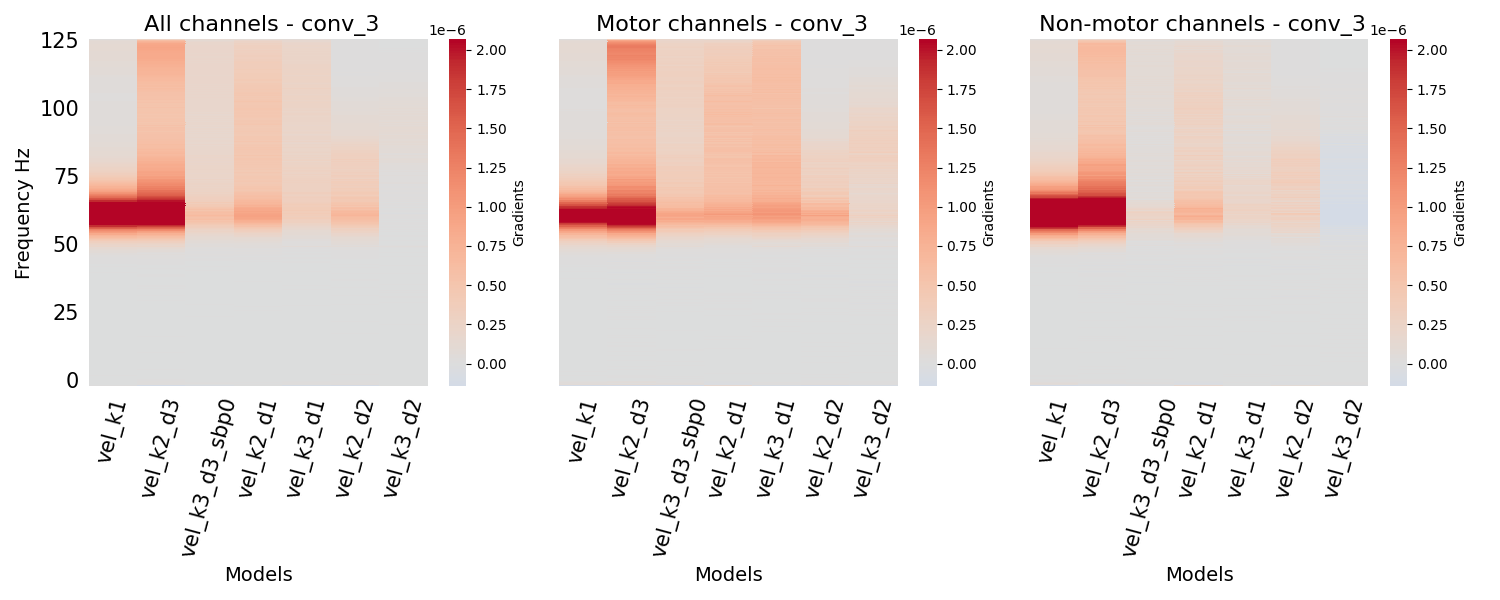
\includegraphics[width=0.9\linewidth]{img/appendix/A/conv-3/hp-m/vel-model-gradients_all_kinds}
   \caption{}
   \label{fig:vel-hp-grads-conv-3}
\end{subfigure}
\end{figure}
\clearpage   

\begin{figure}[!htbp]\ContinuedFloat

\begin{subfigure}[c]{\textwidth}
   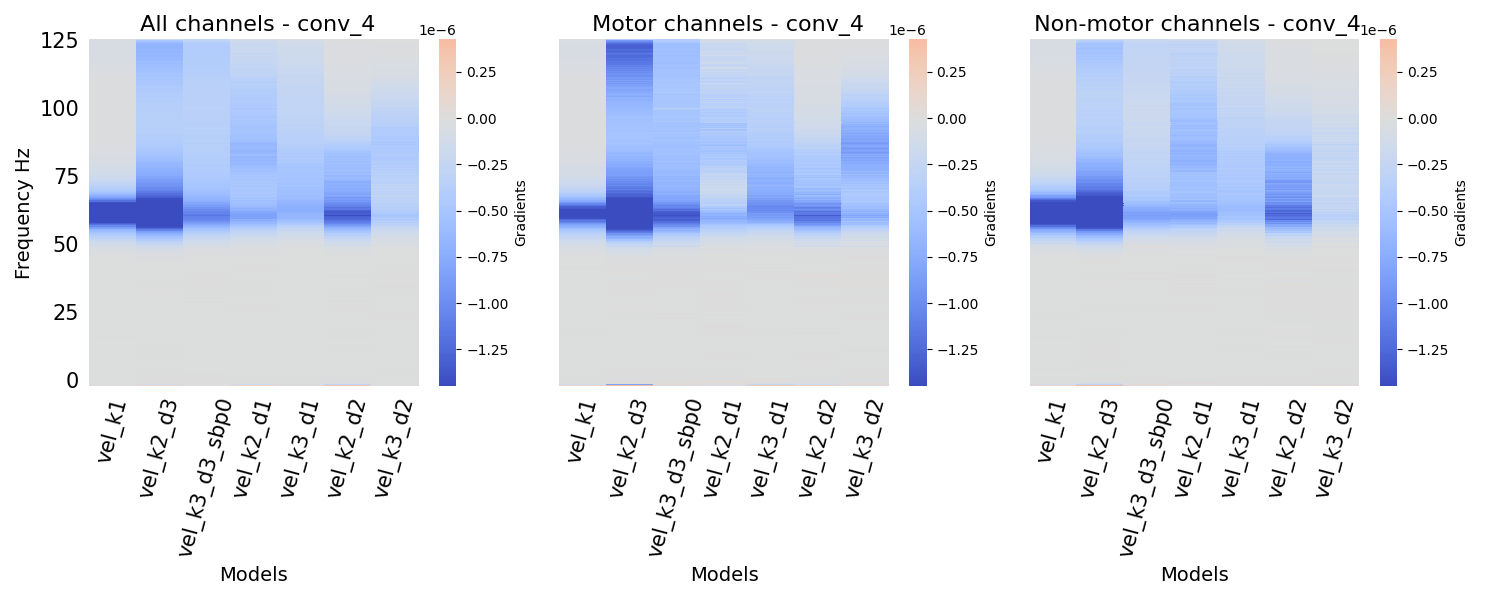
\includegraphics[width=0.9\linewidth]{img/appendix/A/conv-4/hp-m/vel-model_gradients_all_kinds}
   \caption{}
   \label{fig:vel-hp-grads-conv-4}
\end{subfigure}

\begin{subfigure}[d]{\textwidth}
   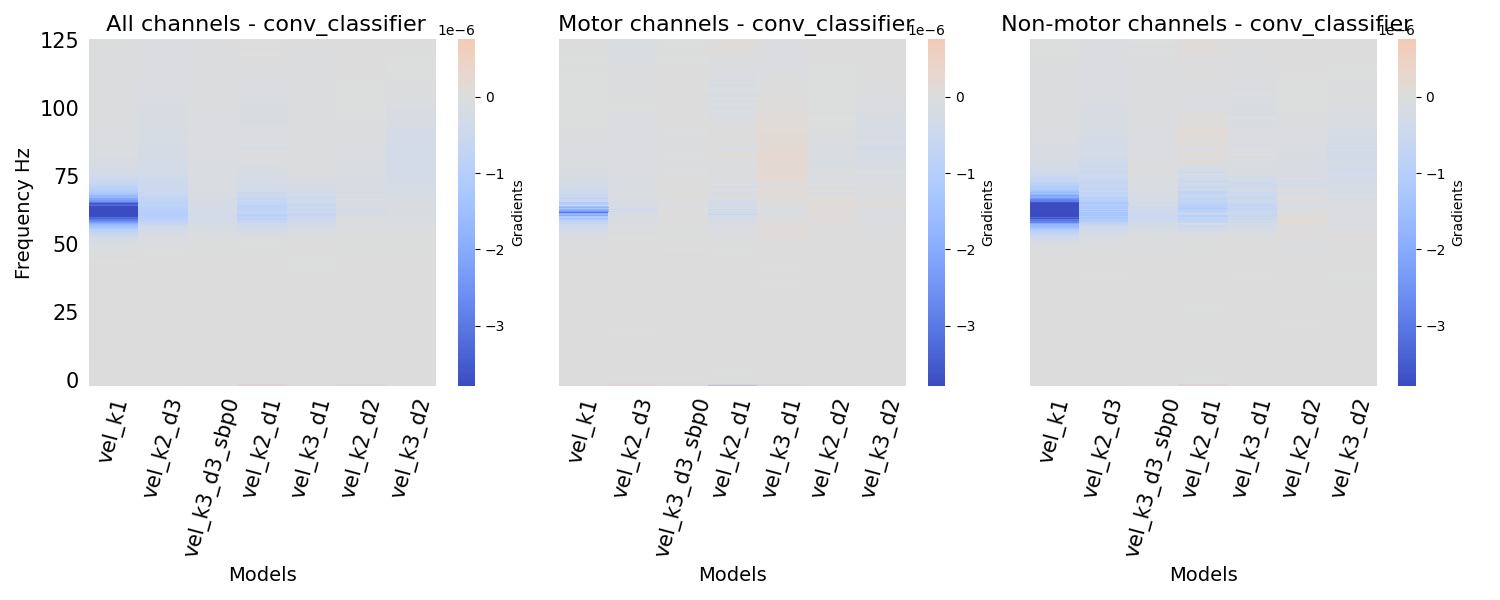
\includegraphics[width=0.9\linewidth]{img/appendix/A/conv-classifier/hp-m/vel-model_gradients_all_kinds}
   \caption{}
   \label{fig:vel-hp-grads-conv-classifier}
\end{subfigure}

\caption[]{Gradients of the different CNN architectures decoding velocity from the high-passed dataset in the original non-shifted setting (causal prediction). \textbf{(a)} shows gradients of the convolutional layer in the second block; \textbf{(b)} shows gradients of the convolutional layer in the third block; \textbf{(c)} shows gradients of the fourth convolutional block; \textbf{(d)} shows gradients of the last convolutional layer - the output layer. All channels include channels that do not belong to motor neither non-motor channel sets. See Section \ref{subsec:ieeg-data-preprocessing}}
\label{fig:vel-hp-grads}
\end{figure}
\clearpage

\section*{Absolute velocity}\label{sec:absolute-velocity-appendixA}

\subsection*{Full dataset}\label{subsec:absVel-full-dataset-appendixA}
\begin{figure}[!htb]
\centering
\begin{subfigure}[a]{\textwidth}
   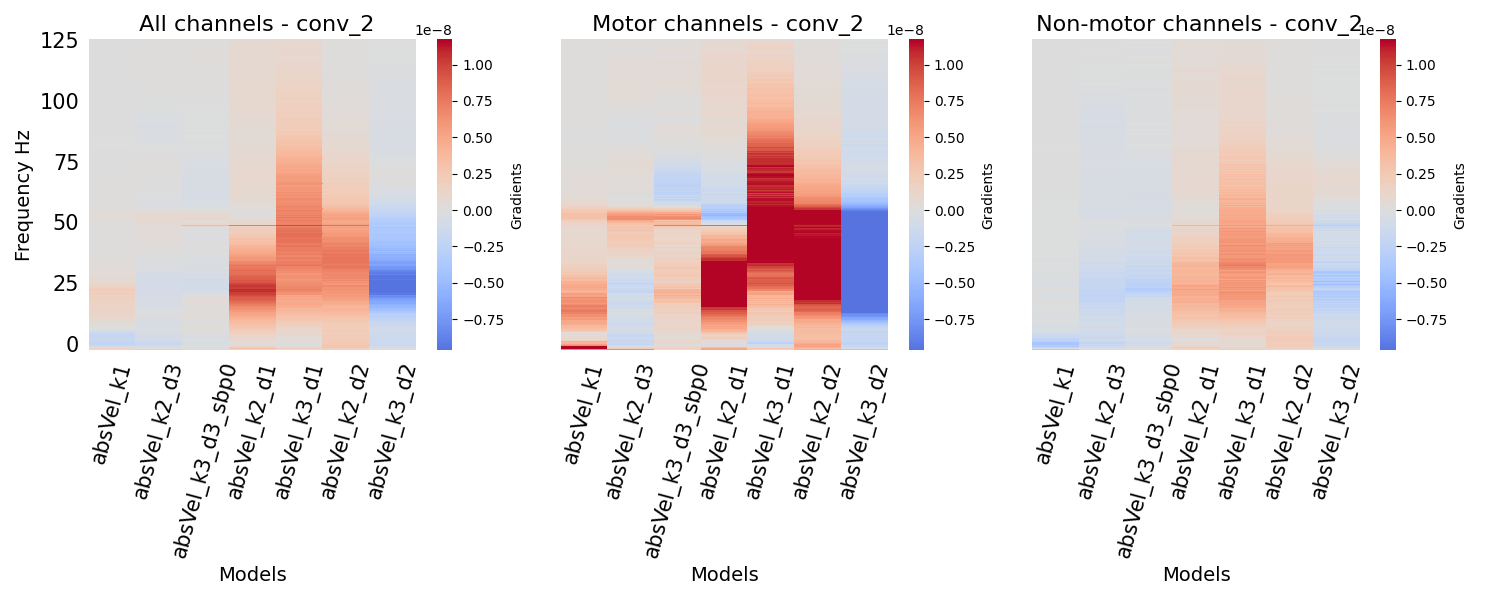
\includegraphics[width=0.9\linewidth]{img/appendix/A/conv-2/m/absVel-model-gradients-all_kinds}
   \caption{}
   \label{fig:absVel-full-grads-conv-2}
\end{subfigure}

\begin{subfigure}[b]{\textwidth}
   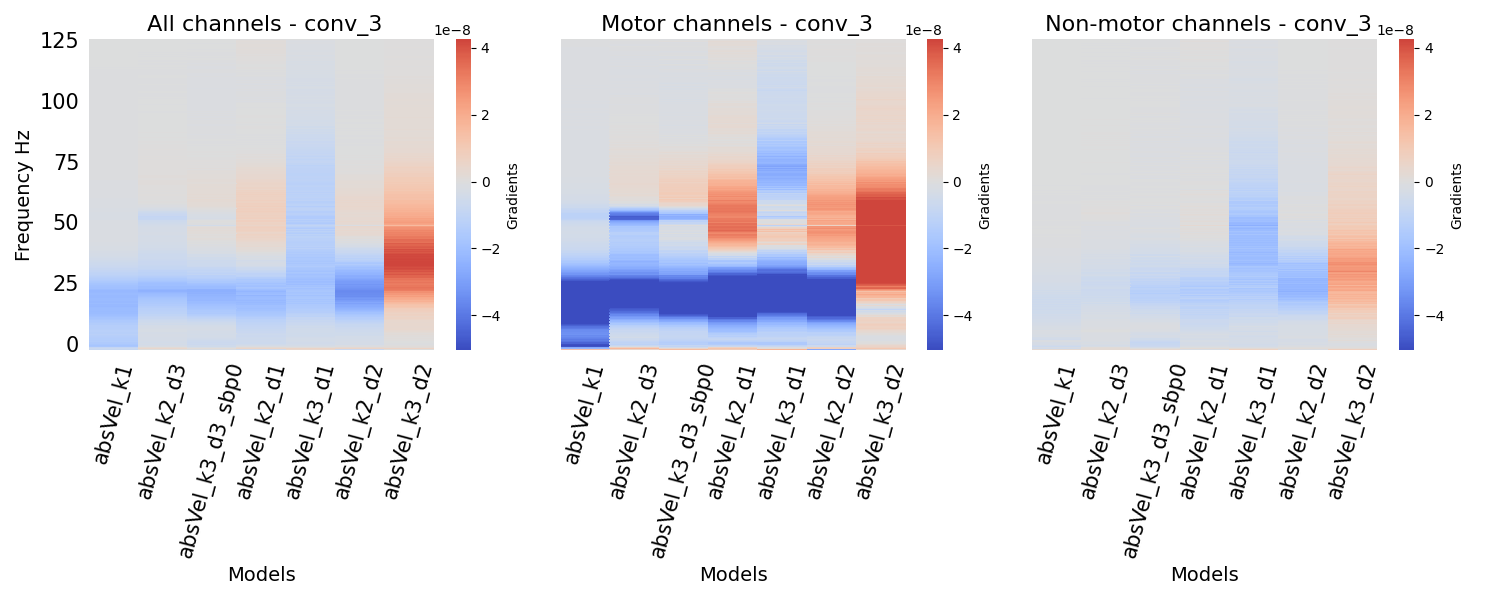
\includegraphics[width=0.9\linewidth]{img/appendix/A/conv-3/m/absVel-model-gradients-all_kinds}
   \caption{}
   \label{fig:absVel-full-grads-conv-3}
\end{subfigure}
\end{figure}
\clearpage   

\begin{figure}[!htbp]\ContinuedFloat

\begin{subfigure}[c]{\textwidth}
   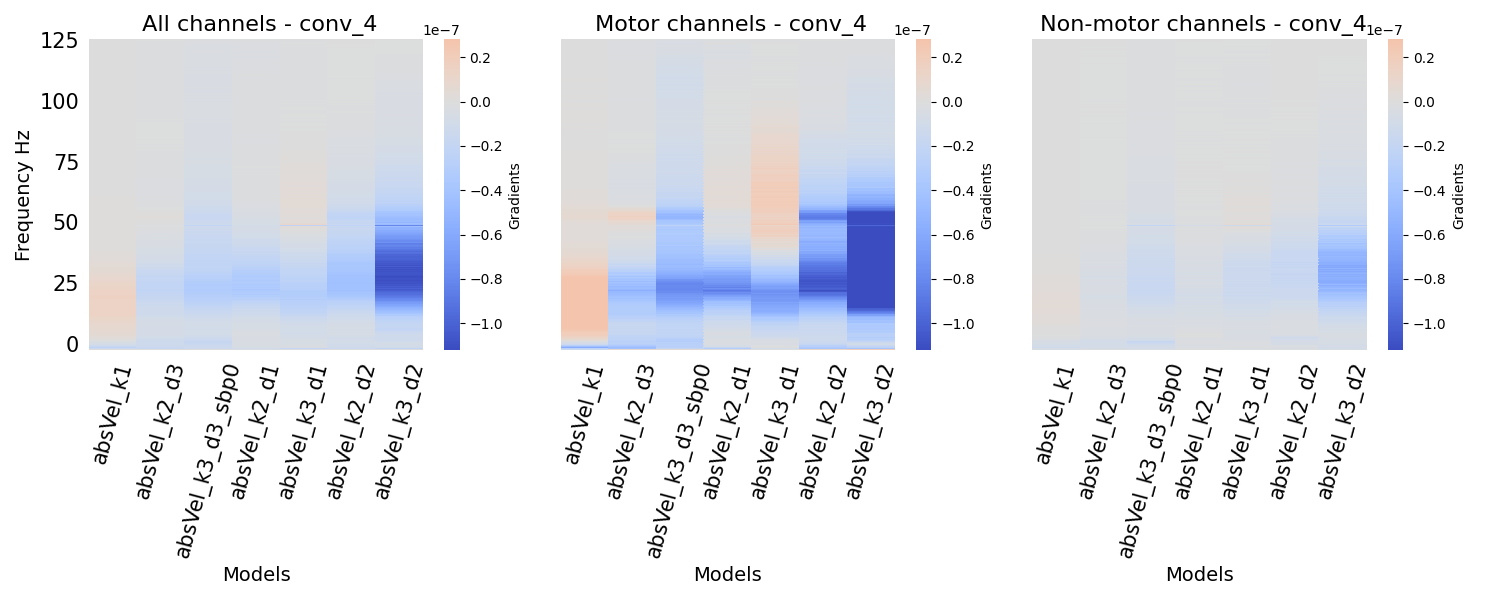
\includegraphics[width=0.9\linewidth]{img/appendix/A/conv-4/m/absVel-model-gradients_all_kinds}
   \caption{}
   \label{fig:absVel-full-grads-conv-4}
\end{subfigure}

\begin{subfigure}[d]{\textwidth}
   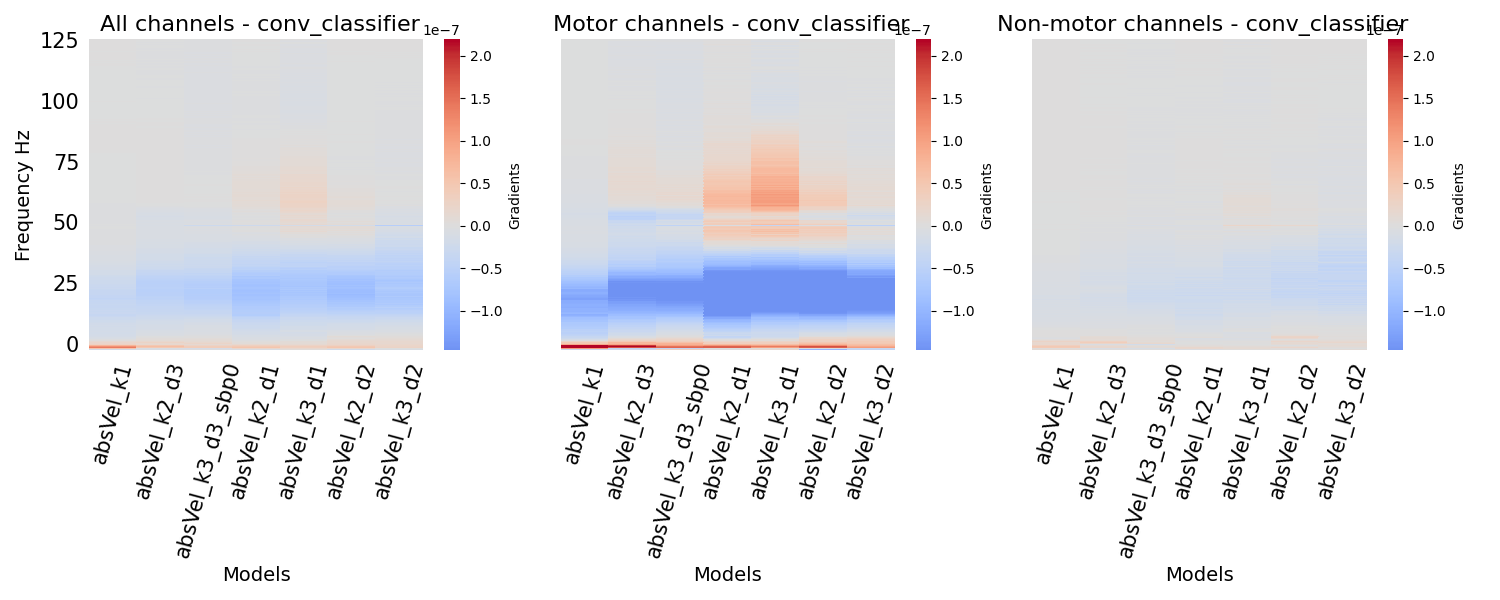
\includegraphics[width=0.9\linewidth]{img/appendix/A/conv-classifier/m/absVel-model-gradients_all_kinds}
   \caption{}
   \label{fig:absVel-full-grads-conv-classifier}
\end{subfigure}

\caption[]{Gradients of the different CNN architectures decoding absolute velocity from the full dataset in the original non-shifted setting (causal prediction). \textbf{(a)} shows gradients of the convolutional layer in the second block; \textbf{(b)} shows gradients of the convolutional layer in the third block; \textbf{(c)} shows gradients of the fourth convolutional block; \textbf{(d)} shows gradients of the last convolutional layer - the output layer. All channels include channels that do not belong to motor neither non-motor channel sets. See Section \ref{subsec:ieeg-data-preprocessing}}
\label{fig:absVel-full-grads}
\end{figure}

\clearpage

\subsection*{High-passed dataset}\label{subsec:absVel-high-passed-dataset-appendixA}
\begin{figure}[!htb]
\centering
\begin{subfigure}[a]{\textwidth}
   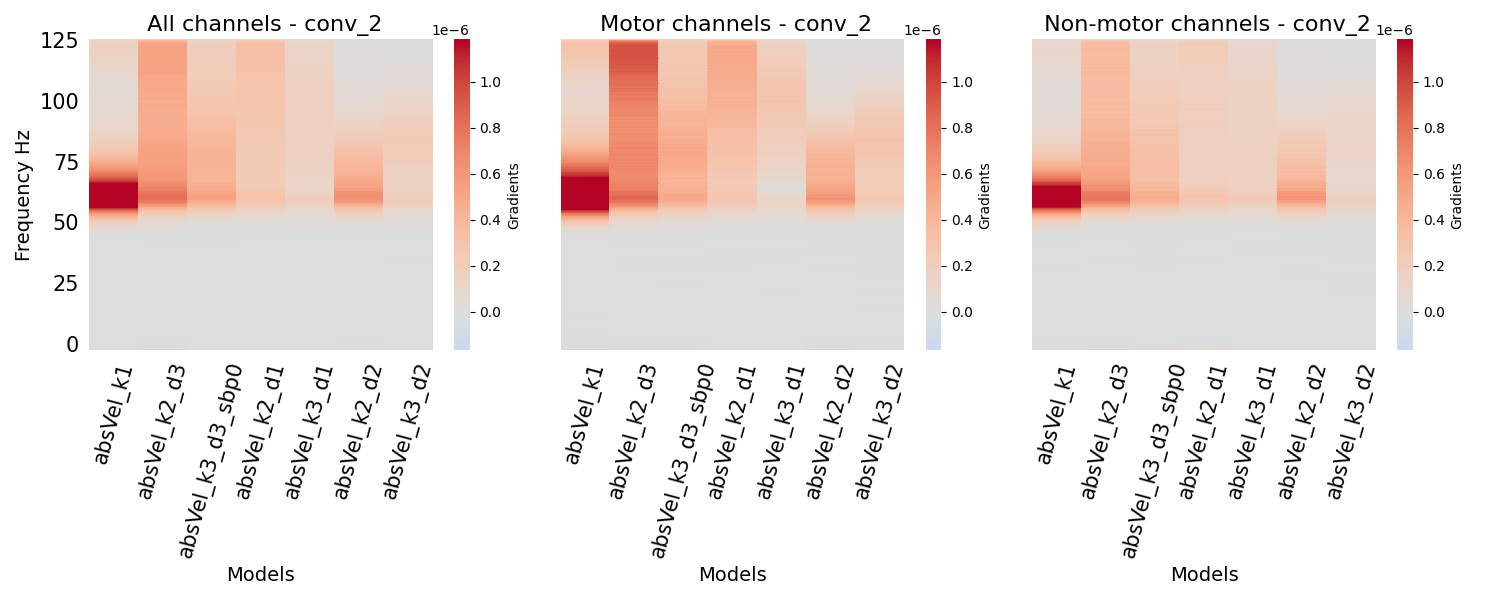
\includegraphics[width=0.9\linewidth]{img/appendix/A/conv-2/hp-m/absVel-model-gradients_all_kinds}
   \caption{}
   \label{fig:absVel-hp-grads-conv-2}
\end{subfigure}

\begin{subfigure}[b]{\textwidth}
   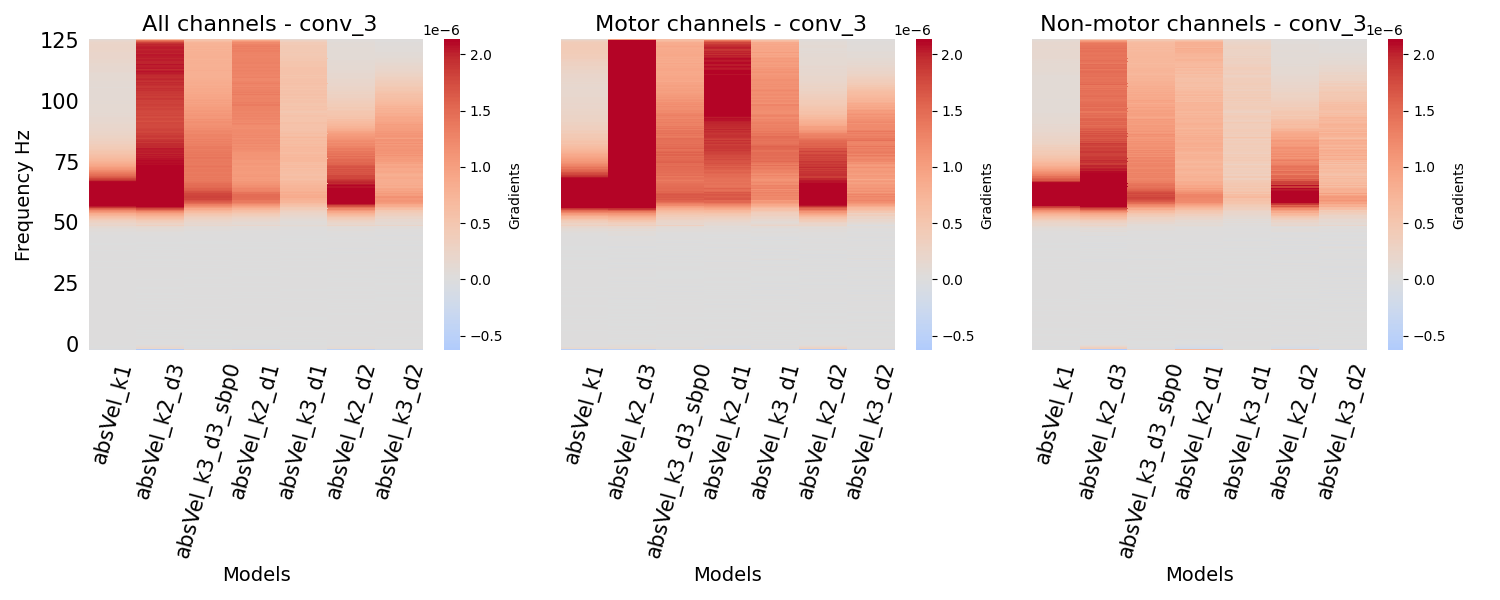
\includegraphics[width=0.9\linewidth]{img/appendix/A/conv-3/hp-m/absVel-model-gradients_all_kinds}
   \caption{}
   \label{fig:absVel-hp-grads-conv-3}
\end{subfigure}
\end{figure}
\clearpage   

\begin{figure}[!htbp]\ContinuedFloat

\begin{subfigure}[c]{\textwidth}
   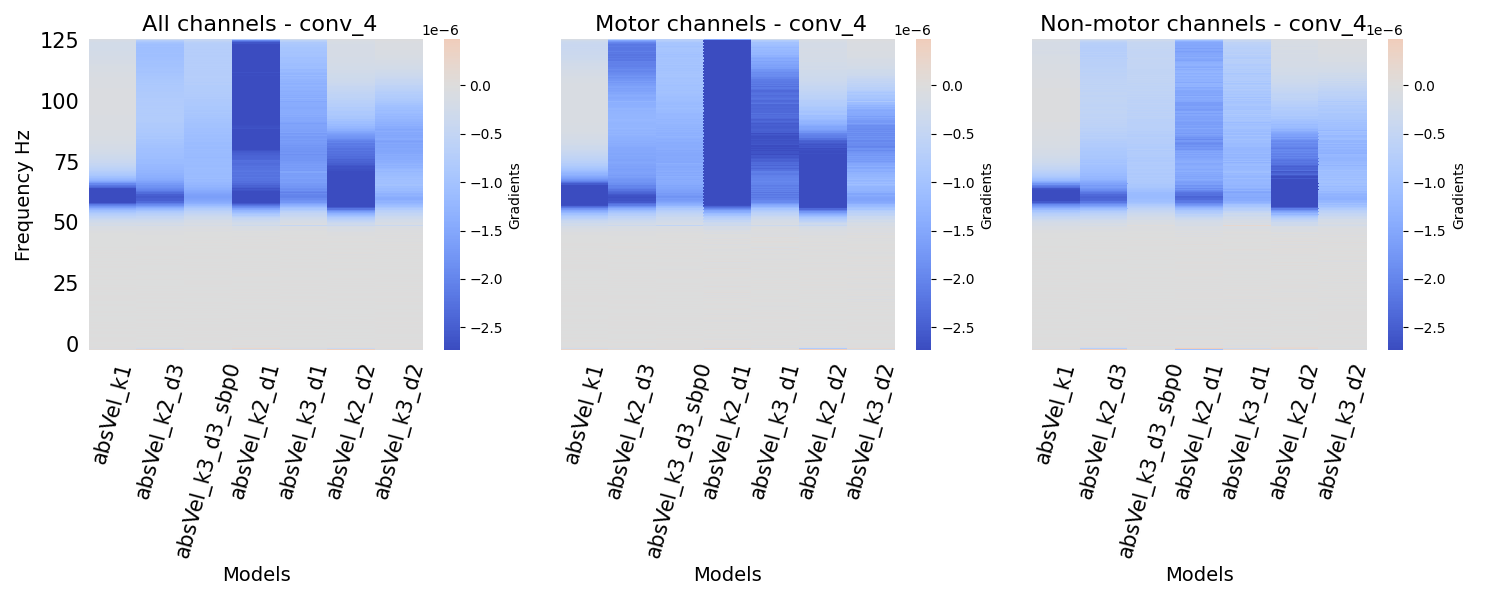
\includegraphics[width=0.9\linewidth]{img/appendix/A/conv-4/hp-m/absVel-model_gradients_all_kinds}
   \caption{}
   \label{fig:absVel-hp-grads-conv-4}
\end{subfigure}


\begin{subfigure}[d]{\textwidth}
   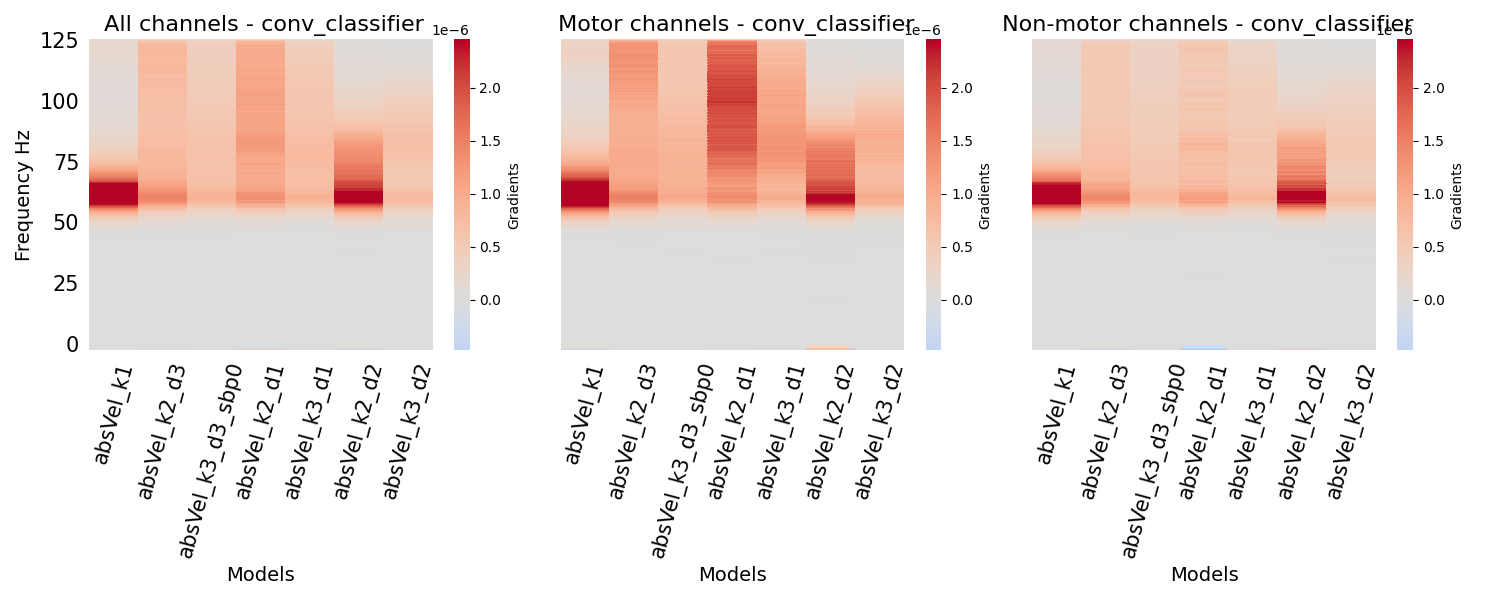
\includegraphics[width=0.9\linewidth]{img/appendix/A/conv-classifier/hp-m/absVel-model_gradients_all_kinds}
   \caption{}
   \label{fig:absVel-hp-grads-conv-classifier}
\end{subfigure}

\caption[]{Gradients of the different CNN architectures decoding absolute velocity from the high-passed dataset in the original non-shifted setting (causal prediction). \textbf{(a)} shows gradients of the convolutional layer in the second block; \textbf{(b)} shows gradients of the convolutional layer in the third block; \textbf{(c)} shows gradients of the fourth convolutional block; \textbf{(d)} shows gradients of the last convolutional layer - the output layer. All channels include channels that do not belong to motor neither non-motor channel sets. See Section \ref{subsec:ieeg-data-preprocessing}}
\label{fig:absVel-hp-grads}
\end{figure}